\subsection{Динамика манипулятора}\label{part_dynamics}

\subsubsection{Общие замечания}
Введем в рассмотрение барицентрические СК $Ox_{ci}y_{ci}z_{ci}$\lefteqn,\footnote{Системы координат, чьи начала совпадают с центрами масс соответствующих звеньев.} где $i=\overline{1,5}$, показанные на рисунке~\ref{img_mass_frames}.
Заметим, что каждая СК $Ox_{ci}y_{ci}z_{ci}$ сонаправлена с $Ox_iy_iz_i$.

\begin{figure}[h!]
	\centering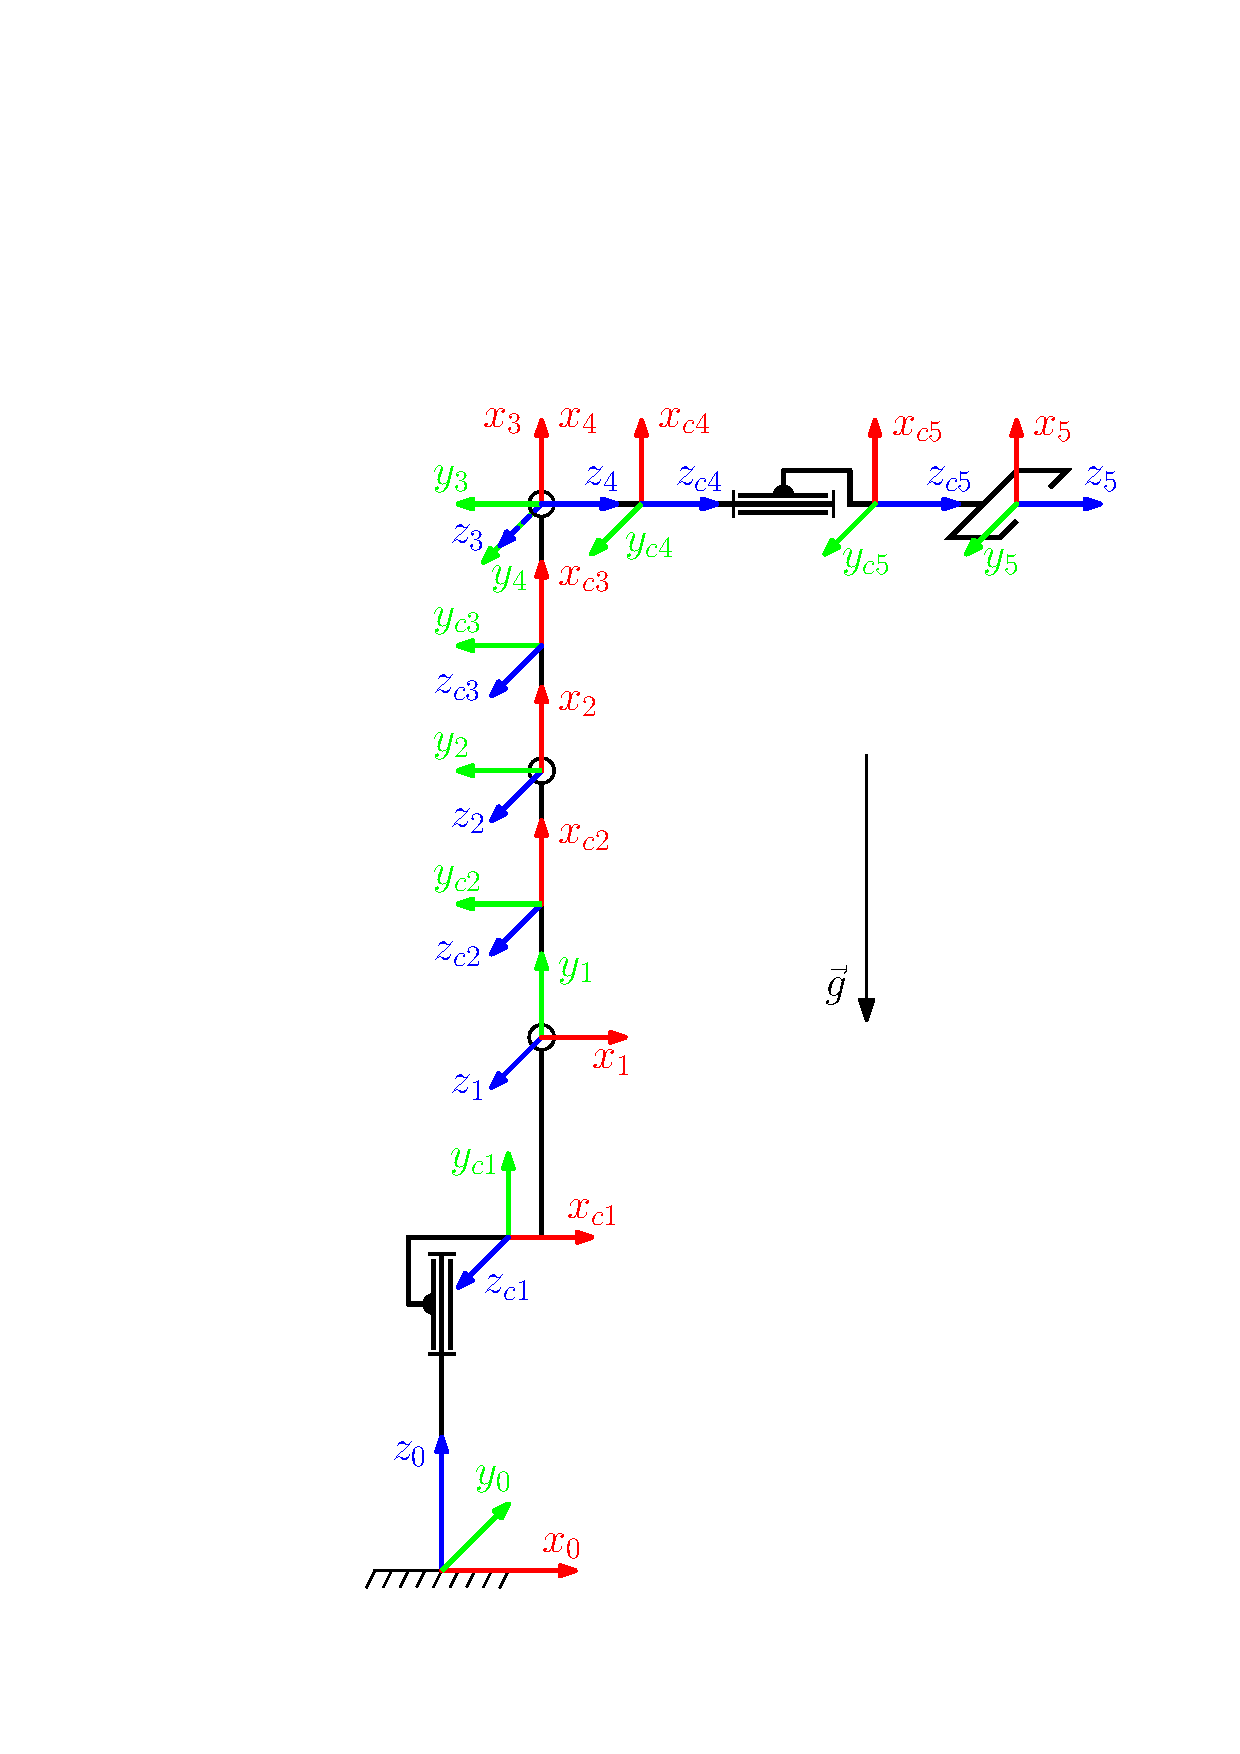
\includegraphics[height=16.5cm]{kinematics_mass_frames.pdf}
	\caption{Положение барицентрических СК и направление вектора $\vec{g}$.}
	\label{img_mass_frames}
\end{figure}

Для описания положения введенных СК воспользуемся следующими векторами:
\begin{equation}
    r^i_{i,\,ci} =
    \begin{bmatrix}
        x_{ci} \\ y_{ci} \\ z_{ci}
    \end{bmatrix}\!\!,\quad i = \overline{1,5},
\end{equation}
где $x_{ci}$, $y_{ci}$ и $z_{ci}$~--- некоторые постоянные величины.

Для компонент тензоров инерции $\mathcal{I}^{ci}_i = const$ введем следующие обозначения:
\begin{equation}
    \mathcal{I}^{ci}_i =
    \begin{bmatrix}
        I_{i,\,xx} & I_{i,\,xy} & I_{i,\,xz} \\
        I_{i,\,xy} & I_{i,\,yy} & I_{i,\,yz} \\
        I_{i,\,xz} & I_{i,\,yz} & I_{i,\,zz}
    \end{bmatrix}\!\!\ldotp
\end{equation}

Заметим, что
\begin{equation}
    g_0 =
    \begin{bmatrix}
        0 \\ 0 \\ -g
    \end{bmatrix}\!\!,
\end{equation}
где $g=9.82\text{ м}/\text{с}^2$.

В~заключении раздела приведем формулы для расчета величин, которые потребуются в дальнейшем (везде $i = \overline{1,5}$):
\begin{itemize}
    \item для расчета $r^0_{0,\,i}$ и ${}^{0}R_i$ (см.~Приложение~\ref{app_ht_matrices}):
        \begin{equation}
            {}^0A_i = {}^0A_1 \cdot {}^1A_2 \cdot \ldots \cdot {}^{i-1}A_i;
        \end{equation}
    \item для расчета $r^0_{0,\,ci}$:
        \begin{equation}
            \begin{bmatrix}
                r^0_{0,\,ci} \\ 1
            \end{bmatrix}
            = {}^0A_i
            \begin{bmatrix}
            r^i_{i,\,ci} \\ 1
            \end{bmatrix}\!\!;
        \end{equation}
    \item для расчета $r^i_{i-1,\,i}$:
        \begin{gather}
            {}^{i-1}A_i \quad \Rightarrow \quad {}^{i-1}R_i,\: r^{i-1}_{i-1,\,i},
            \\
            r^i_{i-1,\,i} = {}^{i-1}R_i^{-1} \!\cdot r^{i-1}_{i-1,\,i};
        \end{gather}
    \item для расчета $z^0_i$:
        \begin{equation}
            z^0_i = {}^{0}R_i \cdot z^i_i = {}^{0}R_i \cdot
            \begin{bmatrix}
                0 \\ 0 \\ 1
            \end{bmatrix}\!\!\ldotp
        \end{equation}
\end{itemize}

\subsubsection{Получение уравнений движения методом Эйлера-Лагранжа}
Потенциальная энергия манипулятора
\begin{equation}
    U = -g_0^T \cdot \sum_{i = 1}^5 m_ir^0_{0,\,ci} =
\end{equation}

Якобианы, устанавливающие в соответствии с формулой
\begin{equation}
    v^0_{ci} = J_{vi}\dot{q}, \quad i = \overline{1,5}
\end{equation}
связь между линейными скоростями центров масс звеньев и вектором~$\dot{q}$:
\begin{gather}
    J_{v1} =
    \begin{bmatrix}
        z^0_0 \times \left( r^0_{0,\,c1} - r^0_{0,\,0}\right) & \nv & \nv & \nv & \nv
    \end{bmatrix}\!\!,
    \\
    J_{v2} =
    \begin{bmatrix}
        z^0_0 \times \left( r^0_{0,\,c2} - r^0_{0,\,0}\right) & z^0_1 \times \left( r^0_{0,\,c2} - r^0_{0,\,1}\right) & \nv & \nv & \nv
    \end{bmatrix}\!\!,
    \\
    J_{v3} =
    \begin{bmatrix}
        z^0_0 \times \left( r^0_{0,\,c3} - r^0_{0,\,0}\right) & z^0_1 \times \left( r^0_{0,\,c3} - r^0_{0,\,1}\right) &
        z^0_2 \times \left( r^0_{0,\,c3} - r^0_{0,\,2}\right) & \nv & \nv
    \end{bmatrix}\!\!,
    \\
    J_{v4} =
    \begin{bmatrix}
        z^0_0 \times \left( r^0_{0,\,c4} - r^0_{0,\,0}\right) \\
        z^0_1 \times \left( r^0_{0,\,c4} - r^0_{0,\,1}\right) \\
        z^0_2 \times \left( r^0_{0,\,c4} - r^0_{0,\,2}\right) \\
        z^0_3 \times \left( r^0_{0,\,c4} - r^0_{0,\,3}\right) \\
        \nv
    \end{bmatrix}^T\!\!\!\!\!,
    \qquad
    J_{v5} =
    \begin{bmatrix}
        z^0_0 \times \left( r^0_{0,\,c5} - r^0_{0,\,0}\right) \\
        z^0_1 \times \left( r^0_{0,\,c5} - r^0_{0,\,1}\right) \\
        z^0_2 \times \left( r^0_{0,\,c5} - r^0_{0,\,2}\right) \\
        z^0_3 \times \left( r^0_{0,\,c5} - r^0_{0,\,3}\right) \\
        z^0_4 \times \left( r^0_{0,\,c5} - r^0_{0,\,4}\right)
    \end{bmatrix}^T\!\!\!\!\!,
\end{gather}
где $\nv = [0\;0\;0]^T$~--- нулевой вектор.

Якобианы, устанавливающие в соответствии с формулой
\begin{equation}
    \omega^0_{ci} = J_{\omega i}\dot{q}, \quad i = \overline{1,5}
\end{equation}
связь между угловыми скоростями звеньев и вектором~$\dot{q}$:
\begin{gather}
    J_{\omega 1} =
    \begin{bmatrix}
        z^0_0 & \nv & \nv & \nv & \nv
    \end{bmatrix}\!\!,
    \qquad
    J_{\omega 2} =
    \begin{bmatrix}
        z^0_0 & z^0_1 & \nv & \nv & \nv
    \end{bmatrix}\!\!,
    \\
    J_{\omega 3} =
    \begin{bmatrix}
         z^0_0 & z^0_1 & z^0_2 & \nv & \nv
    \end{bmatrix}\!\!,
    \qquad
    J_{\omega 4} =
    \begin{bmatrix}
        z^0_0 & z^0_1 & z^0_2 & z^0_3 & \nv
    \end{bmatrix}\!\!,
    \\
    J_{\omega 5} =
    \begin{bmatrix}
        z^0_0 & z^0_1 & z^0_2 & z^0_3 & z^0_4
    \end{bmatrix}\!\!\ldotp
\end{gather}

Кинетическая энергия манипулятора:
\begin{equation}
    K = \frac{1}{2}\, \dot{q}^T \left( \sum_{i=1}^5 \left( m_i J_{vi}^T J_{vi} + J_{\omega i}^T \, {}^0\!R_i \, \mathcal{I}^{ci}_i \, {}^0\!R_i^T J_{\omega i} \right) \right) \dot{q} =
\end{equation}

Функция Лагранжа
\begin{equation}
    L = K - U\ldotp
\end{equation}

Уравнения движения робота:
\begin{equation}
    \frac{d}{dt}\frac{\partial L}{\partial\dot{q_i}} - \frac{\partial L}{\partial q_i} = \tau_i, \quad i = \overline{1,5} \qquad \Rightarrow
\end{equation}
\begin{equation}\label{eq_system_of_equations_1}
    \Rightarrow \quad
	\left\{
	\begin{aligned}
		\!& = \tau_1\\
		\!& = \tau_2\\
		\!& = \tau_3\\
		\!& = \tau_4\\
		\!& = \tau_5
	\end{aligned}
	\right.
\end{equation}

\subsubsection{Получение уравнений движения методом Ньютона-Эйлера}
Для определения необходимых скоростей и ускорений с учетом <<начальных условий>>:
\begin{equation}
    \omega^0_0=0, \quad \dot\omega^0_0=0, \quad a^0_0=0,
\end{equation}
служат следующие рекурсивные формулы:
\begin{equation}
    \omega^i_i = {}^{i-1}R_i^T\left(\omega^{i-1}_{i-1} + \dot{q_i}z^{i-1}_{i-1}\right)\!,
\end{equation}
\begin{equation}
    \dot{\omega}^i_i = {}^{i-1}R_i^T\left(\dot{\omega}^{i-1}_{i-1} + \ddot{q_i}z^{i-1}_{i-1} + \dot{q}_i\omega^{i-1}_{i-1} \times z^{i-1}_{i-1}\right)\!,
\end{equation}
\begin{equation}
    a^i_i = {}^{i-1}R_i^Ta^{i-1}_{i-1} + \dot{\omega}^i_i \times r^i_{i-1,\,i} + \omega^i_i \times \left(\omega^i_i \times r^i_{i-1,\,i}\right)\!,
\end{equation}
\begin{equation}
    a^i_{ci} = a^i_i + \dot{\omega}^i_i \times r^i_{i,\,ci} + \omega^i_i \times \left(\omega^i_i \times r^i_{i,\,ci}\right)\!\ldotp
\end{equation}
Применив их, получим:
\begin{gather}
    \omega^1_1 = {}^{0}R_1^T\left(\omega^{0}_{0} + \dot{q_1}z^{0}_{0}\right) =
    \begin{bmatrix}
        ? \\ ? \\ ?
    \end{bmatrix}\!\!,
    \\
    \dot{\omega}^1_1 = {}^{0}R_1^T\left(\dot{\omega}^0_0 + \ddot{q_1}z^0_0 + \dot{q}_1\omega^0_0 \times z^0_0 \right) =
    \begin{bmatrix}
        ? \\ ? \\ ?
    \end{bmatrix}\!\!,
    \\
    a^1_1 = {}^{0}R_1^Ta^0_0 + \dot{\omega}^1_1 \times r^1_{0,\,1} + \omega^1_1 \times \left(\omega^1_1 \times r^1_{0,\,1}\right) =
    \begin{bmatrix}
        ? \\ ? \\ ?
    \end{bmatrix}\!\!,
    \\
    a^1_{c1} = a^1_1 + \dot{\omega}^1_1 \times r^1_{1,\,c1} + \omega^1_1 \times \left(\omega^1_1 \times r^1_{1,\,c1}\right) =
    \begin{bmatrix}
        ? \\ ? \\ ?
    \end{bmatrix}\!\!,
    \\
    \omega^2_2 = {}^{1}R_2^T\left(\omega^{1}_{1} + \dot{q_2}z^{1}_{1}\right) =
    \begin{bmatrix}
        ? \\ ? \\ ?
    \end{bmatrix}\!\!,
    \\
    \dot{\omega}^2_2 = {}^{1}R_2^T\left(\dot{\omega}^1_1 + \ddot{q_2}z^1_1 + \dot{q}_2\omega^1_1 \times z^1_1 \right) =
    \begin{bmatrix}
        ? \\ ? \\ ?
    \end{bmatrix}\!\!,
    \\
    \ldots\notag
\end{gather}


Для определения сил и моментов, с которыми звенья робота действуют друг на друга, с учетом <<начальных условий>>:
\begin{equation}
    f^5_6=0, \qquad \tau^5_6=0, \qquad g_5= {}^0R_5^T g_0,
\end{equation}
используются следующие рекурсивные формулы:
\begin{equation}
    f^i_i = f^i_{i+1} + m_i(a^i_{ci} - g_i),
\end{equation}
\begin{equation}
    \tau^i_i = \tau^i_{i+1} - f^i_i\times(r^i_{i-1,\,i} - r^i_{i,\,ci}) + f^i_{i+1} \times r^i_{i,\,ci} + \mathcal{I}^{ci}_i\dot\omega^i_i + \omega_i^i\times(\mathcal{I}^{ci}_i\omega_i^i)\ldotp
\end{equation}
\begin{equation}
    g_{i-1} = {}^{i-1}R_ig_i,
    \qquad
    f^{i-1}_i = {}^{i-1}R_{i}f^{i}_{i},
    \qquad
    \tau^{i-1}_{i} = {}^{i-1}R_{i}\tau^{i}_{i}\ldotp
\end{equation}
Воспользовавшись ими, получим:
\begin{gather}
    g_5= {}^0R_5^T g_0 =
    \begin{bmatrix}
        ? \\ ? \\ ?
    \end{bmatrix}\!\!,
    \\
    f^5_5 = f^5_{6} + m_5(a^5_{c5} - g_5) =
    \begin{bmatrix}
        ? \\ ? \\ ?
    \end{bmatrix}\!\!,
    \\
    \tau^5_5 = \tau^5_6 - f^5_5\times(r^5_{4,\,5} - r^5_{5,\,c5}) + f^5_6 \times r^5_{5,\,c5} + \mathcal{I}^{c5}_5\dot\omega^5_5 + \omega_5^5\times(\mathcal{I}^{c5}_5\omega_5^5) =
    \begin{bmatrix}
        ? \\ ? \\ ?
    \end{bmatrix}\!\!,
    \\
    g_4 = {}^4R_5g_5 =
    \begin{bmatrix}
        ? \\ ? \\ ?
    \end{bmatrix}\!\!,
    \quad
    f^4_5 = {}^{4}R_5f^5_5 =
    \begin{bmatrix}
        ? \\ ? \\ ?
    \end{bmatrix}\!\!,
    \quad
    \tau^4_5 = {}^{4}R_5\tau^5_5 =
    \begin{bmatrix}
        ? \\ ? \\ ?
    \end{bmatrix}\!\!,
    \\
    f^4_4 = f^4_{5} + m_4(a^4_{c4} - g_4) =
    \begin{bmatrix}
        ? \\ ? \\ ?
    \end{bmatrix}\!\!,
    \\
    \ldots \notag
\end{gather}

Обобщенные моменты, а вместе с тем и уравнения движения манипулятора могут быть найдены по формуле:
\begin{equation}
    \tau_i = (\tau^i_i)^T \: {}^{i-1}\!R_i^T z^{i-1}_{i-1}	, \quad i = \overline{1,5}\ldotp
\end{equation}
С~учетом их получаем, что
\begin{equation}\label{eq_system_of_equations_2}
	\left\{
	\begin{aligned}
		\!&\tau_1 = \\
		\!&\tau_2 = \\
		\!&\tau_3 = \\
		\!&\tau_4 = \\
		\!&\tau_5 =
	\end{aligned}
	\right.
\end{equation}

\subsubsection{Уравнение движения в матричном виде}
Уравнение движения системы в матричном виде, записанное на основании~\eqref{eq_system_of_equations_1} или~\eqref{eq_system_of_equations_2}, примет вид
\begin{equation}\label{eq:eq_of_motion}
    M(q)\ddot{q} + C(q,\dot{q}) + G(q) = \tau,
\end{equation}
где $M(q)$~--- матрица инерции, $C(q,\dot{q})$~--- вектор центробежных и Кориолисовых сил, $G(q)$~--- вектор гравитации, $\tau$~--- вектор обобщенных сил и моментов, равные
\begin{gather}
    \quad
    M(q) =
    \begin{bmatrix}
        ?
    \end{bmatrix}\!\!,
    \quad
    C(q,\dot{q}) =
    \begin{bmatrix}
        ?
    \end{bmatrix}\!\!,
    \\
    G(q) =
    \begin{bmatrix}
        ?
    \end{bmatrix}\!\!,
    \qquad
    \tau =
    \begin{bmatrix}
        \tau_1 \\ \tau_2 \\ \tau_3 \\ \tau_4 \\ \tau_5 \\ \tau_6
    \end{bmatrix}\!\!\ldotp
\end{gather}

\newpage
